\section{Pre-requisites}

\begin{frame}{Prerequisites}
	\begin{center}
		\Huge
		Time Series
	\end{center}
\end{frame}
	
\begin{frame}[allowframebreaks]
	\frametitle{Examples}
	\begin{figure}[H]
		\centering
		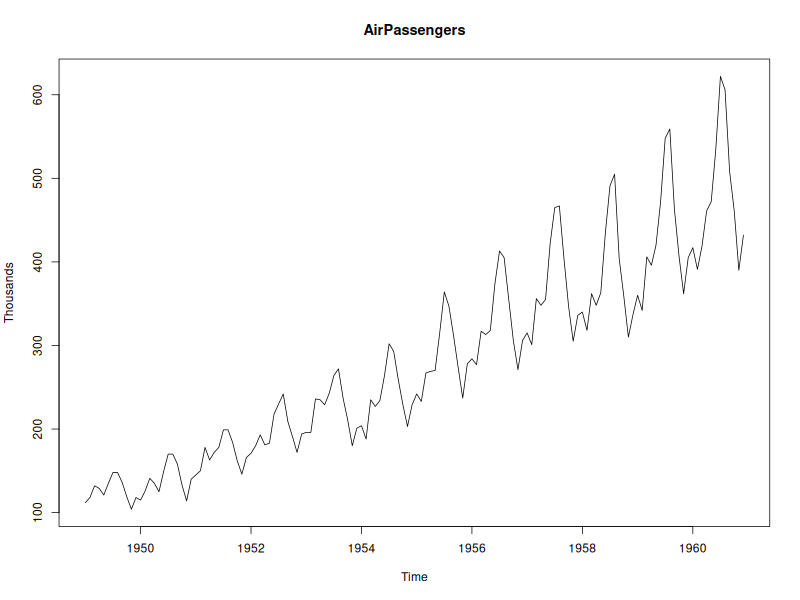
\includegraphics[width=0.75\linewidth]{images/AirPassengers__plot.png}
		\caption{Example of a \textbf{non-stationary} time series}
	\end{figure}
	\small
	Refer: Monthly airline passengers (1949-1960) [R-datasets]
	
	\framebreak
	
	\begin{figure}[H]
		\centering
		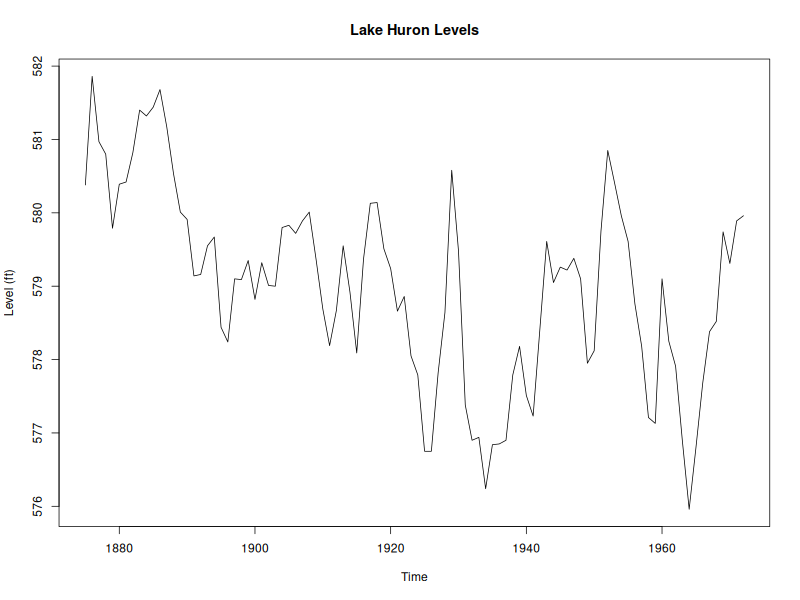
\includegraphics[width=0.75\linewidth]{images/LakeHuron_plot.png}
		\caption{Example of a \textbf{nearly stationary} time series}
	\end{figure}
	\small
	Refer: Annual level of Lake Huron (1875-1972) [R-datasets]
	
	\framebreak
	
	\begin{figure}[H]
		\centering
		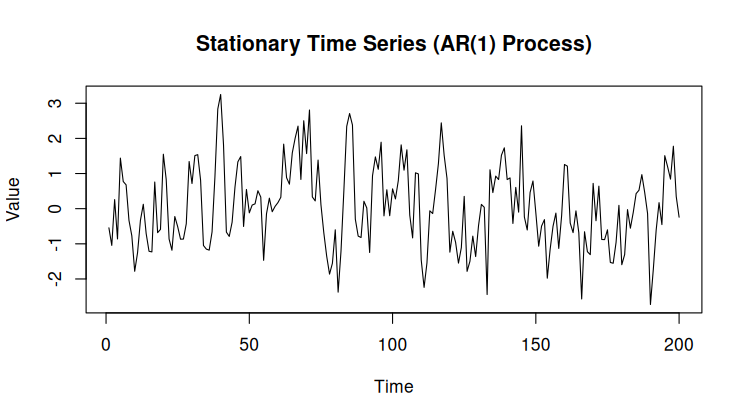
\includegraphics[width=0.75\linewidth]{notes/stationary_ts.png}
		\caption{Example of a \textbf{stationary} time series}
	\end{figure}
	\small
	It is AR(1) process.
	
	\framebreak
\end{frame}

\begin{frame}[allowframebreaks]
	\frametitle{Pre-requisites}
	\textbf{What is a stationary time series?}
	
	A stationary time series is one whose statistical properties do not change over time. Formally, a time series {$y_t$} is weakly stationary if:
	\begin{itemize}
		\item Constant mean: E[$y_t$] = $\mu$ $\forall\ t$
		\item E[$y_t^2$] $< \infty$
		\item Covariance depends only on lag: Cov($y_t, y_{t-k}$) = $\gamma_k$, which only depends on the lag $k$ and not on time $t$.
	\end{itemize}
	
	\framebreak
	
	\textbf{Unit root geometrically}
	
	\begin{itemize}
		\item A unit root means one of these roots lie on the unit circle, i.e., $|z|=1$. Eg: $y_t = \phi y_{t-1} + a_t$.
		
		\item Characteristic equation: $1 - \phi B = 0 \implies B = \frac{1}{\phi}$.
		
		\begin{itemize}
			\item If $|\phi|<1$, then the root lies outside the unit circle $\implies$ stationary.
			
			\item If $|\phi|=1$, then the root lies exactly on the unit circle $\implies$ unit root non-stationary.
			
			\item If $|\phi|>1$, then the root lies outside the unit circle $\implies$ explosive series.
		\end{itemize}
	\end{itemize}
	
	\framebreak
	
	\begin{table}[h!]
		\centering
		\tiny
		\begin{tabular}{llll}
			\toprule
			\textbf{Property} & \textbf{Stationary} & \textbf{Unit Root} & \textbf{Differenced} \\
			& & \textbf{(Nonstationary)} & \textbf{(Stationary)}\\
			
			\midrule
			Equation & $y_t = 0.5y_{t-1} + a_t$ & $y_t = y_{t-1} + a_t$ & $\Delta y_t = a_t$ \\
			
			Process Type & AR(1), $I(0)$ & Random Walk, $I(1)$ & White Noise, $I(0)$ \\
			
			Stationarity & Yes & No & Yes \\
			\bottomrule
		\end{tabular}
		\caption{Comparison of stationary, unit root, and differenced time series.}
		\label{tab:ts_comparison}
	\end{table}
\end{frame}
